\documentclass[12pt]{beamer}
\usetheme{default}
\usepackage[labelformat=empty]{subfig}

\usepackage{amsfonts}
\usepackage{stmaryrd}
\usepackage{upgreek}
\usepackage{url}


\usepackage[greek,english]{babel}


\DeclareMathAlphabet{\mathkw}{OT1}{cmss}{bx}{n}

\usepackage{color}
\newcommand{\redFG}[1]{\textcolor[rgb]{0.6,0,0}{#1}}
\newcommand{\greenFG}[1]{\textcolor[rgb]{0,0.4,0}{#1}}
\newcommand{\blueFG}[1]{\textcolor[rgb]{0,0,0.8}{#1}}
\newcommand{\orangeFG}[1]{\textcolor[rgb]{0.8,0.4,0}{#1}}
\newcommand{\purpleFG}[1]{\textcolor[rgb]{0.4,0,0.4}{#1}}
\newcommand{\yellowFG}[1]{\textcolor{yellow}{#1}}
\newcommand{\brownFG}[1]{\textcolor[rgb]{0.5,0.2,0.2}{#1}}
\newcommand{\blackFG}[1]{\textcolor[rgb]{0,0,0}{#1}}
\newcommand{\whiteFG}[1]{\textcolor[rgb]{1,1,1}{#1}}
\newcommand{\yellowBG}[1]{\colorbox[rgb]{1,1,0.2}{#1}}
\newcommand{\brownBG}[1]{\colorbox[rgb]{1.0,0.7,0.4}{#1}}

\newcommand{\ColourStuff}{
  \newcommand{\red}{\redFG}
  \newcommand{\green}{\greenFG}
  \newcommand{\blue}{\blueFG}
  \newcommand{\orange}{\orangeFG}
  \newcommand{\purple}{\purpleFG}
  \newcommand{\yellow}{\yellowFG}
  \newcommand{\brown}{\brownFG}
  \newcommand{\black}{\blackFG}
  \newcommand{\white}{\whiteFG}
}

\newcommand{\MonochromeStuff}{
  \newcommand{\red}{\blackFG}
  \newcommand{\green}{\blackFG}
  \newcommand{\blue}{\blackFG}
  \newcommand{\orange}{\blackFG}
  \newcommand{\purple}{\blackFG}
  \newcommand{\yellow}{\blackFG}
  \newcommand{\brown}{\blackFG}
  \newcommand{\black}{\blackFG}
  \newcommand{\white}{\blackFG}
}

\ColourStuff

\newcommand{\K}[1]{\yellow{\mathsf{#1}}}
\newcommand{\I}[1]{\green{\mathsf{#1}}}
\newcommand{\D}[1]{\blue{\mathsf{#1}}}
\newcommand{\C}[1]{\red{\mathsf{#1}}}
\newcommand{\F}[1]{\green{\mathsf{#1}}}
\newcommand{\V}[1]{\purple{\mathit{#1}}}

\usepackage{ucs}
\usepackage[utf8x]{inputenc}

%% ODER: format ==         = "\mathrel{==}"
%% ODER: format /=         = "\neq "
%
%
\makeatletter
\@ifundefined{lhs2tex.lhs2tex.sty.read}%
  {\@namedef{lhs2tex.lhs2tex.sty.read}{}%
   \newcommand\SkipToFmtEnd{}%
   \newcommand\EndFmtInput{}%
   \long\def\SkipToFmtEnd#1\EndFmtInput{}%
  }\SkipToFmtEnd

\newcommand\ReadOnlyOnce[1]{\@ifundefined{#1}{\@namedef{#1}{}}\SkipToFmtEnd}
\usepackage{amstext}
\usepackage{amssymb}
\usepackage{stmaryrd}
\DeclareFontFamily{OT1}{cmtex}{}
\DeclareFontShape{OT1}{cmtex}{m}{n}
  {<5><6><7><8>cmtex8
   <9>cmtex9
   <10><10.95><12><14.4><17.28><20.74><24.88>cmtex10}{}
\DeclareFontShape{OT1}{cmtex}{m}{it}
  {<-> ssub * cmtt/m/it}{}
\newcommand{\texfamily}{\fontfamily{cmtex}\selectfont}
\DeclareFontShape{OT1}{cmtt}{bx}{n}
  {<5><6><7><8>cmtt8
   <9>cmbtt9
   <10><10.95><12><14.4><17.28><20.74><24.88>cmbtt10}{}
\DeclareFontShape{OT1}{cmtex}{bx}{n}
  {<-> ssub * cmtt/bx/n}{}
\newcommand{\tex}[1]{\text{\texfamily#1}}	% NEU

\newcommand{\Sp}{\hskip.33334em\relax}


\newcommand{\Conid}[1]{\mathit{#1}}
\newcommand{\Varid}[1]{\mathit{#1}}
\newcommand{\anonymous}{\kern0.06em \vbox{\hrule\@width.5em}}
\newcommand{\plus}{\mathbin{+\!\!\!+}}
\newcommand{\bind}{\mathbin{>\!\!\!>\mkern-6.7mu=}}
\newcommand{\rbind}{\mathbin{=\mkern-6.7mu<\!\!\!<}}% suggested by Neil Mitchell
\newcommand{\sequ}{\mathbin{>\!\!\!>}}
\renewcommand{\leq}{\leqslant}
\renewcommand{\geq}{\geqslant}
\usepackage{polytable}

%mathindent has to be defined
\@ifundefined{mathindent}%
  {\newdimen\mathindent\mathindent\leftmargini}%
  {}%

\def\resethooks{%
  \global\let\SaveRestoreHook\empty
  \global\let\ColumnHook\empty}
\newcommand*{\savecolumns}[1][default]%
  {\g@addto@macro\SaveRestoreHook{\savecolumns[#1]}}
\newcommand*{\restorecolumns}[1][default]%
  {\g@addto@macro\SaveRestoreHook{\restorecolumns[#1]}}
\newcommand*{\aligncolumn}[2]%
  {\g@addto@macro\ColumnHook{\column{#1}{#2}}}

\resethooks

\newcommand{\onelinecommentchars}{\quad-{}- }
\newcommand{\commentbeginchars}{\enskip\{-}
\newcommand{\commentendchars}{-\}\enskip}

\newcommand{\visiblecomments}{%
  \let\onelinecomment=\onelinecommentchars
  \let\commentbegin=\commentbeginchars
  \let\commentend=\commentendchars}

\newcommand{\invisiblecomments}{%
  \let\onelinecomment=\empty
  \let\commentbegin=\empty
  \let\commentend=\empty}

\visiblecomments

\newlength{\blanklineskip}
\setlength{\blanklineskip}{0.66084ex}

\newcommand{\hsindent}[1]{\quad}% default is fixed indentation
\let\hspre\empty
\let\hspost\empty
\newcommand{\NB}{\textbf{NB}}
\newcommand{\Todo}[1]{$\langle$\textbf{To do:}~#1$\rangle$}

\EndFmtInput
\makeatother
%
%
%
%
%
%
% This package provides two environments suitable to take the place
% of hscode, called "plainhscode" and "arrayhscode". 
%
% The plain environment surrounds each code block by vertical space,
% and it uses \abovedisplayskip and \belowdisplayskip to get spacing
% similar to formulas. Note that if these dimensions are changed,
% the spacing around displayed math formulas changes as well.
% All code is indented using \leftskip.
%
% Changed 19.08.2004 to reflect changes in colorcode. Should work with
% CodeGroup.sty.
%
\ReadOnlyOnce{polycode.fmt}%
\makeatletter

\newcommand{\hsnewpar}[1]%
  {{\parskip=0pt\parindent=0pt\par\vskip #1\noindent}}

% can be used, for instance, to redefine the code size, by setting the
% command to \small or something alike
\newcommand{\hscodestyle}{}

% The command \sethscode can be used to switch the code formatting
% behaviour by mapping the hscode environment in the subst directive
% to a new LaTeX environment.

\newcommand{\sethscode}[1]%
  {\expandafter\let\expandafter\hscode\csname #1\endcsname
   \expandafter\let\expandafter\endhscode\csname end#1\endcsname}

% "compatibility" mode restores the non-polycode.fmt layout.

\newenvironment{compathscode}%
  {\par\noindent
   \advance\leftskip\mathindent
   \hscodestyle
   \let\\=\@normalcr
   \let\hspre\(\let\hspost\)%
   \pboxed}%
  {\endpboxed\)%
   \par\noindent
   \ignorespacesafterend}

\newcommand{\compaths}{\sethscode{compathscode}}

% "plain" mode is the proposed default.
% It should now work with \centering.
% This required some changes. The old version
% is still available for reference as oldplainhscode.

\newenvironment{plainhscode}%
  {\hsnewpar\abovedisplayskip
   \advance\leftskip\mathindent
   \hscodestyle
   \let\hspre\(\let\hspost\)%
   \pboxed}%
  {\endpboxed%
   \hsnewpar\belowdisplayskip
   \ignorespacesafterend}

\newenvironment{oldplainhscode}%
  {\hsnewpar\abovedisplayskip
   \advance\leftskip\mathindent
   \hscodestyle
   \let\\=\@normalcr
   \(\pboxed}%
  {\endpboxed\)%
   \hsnewpar\belowdisplayskip
   \ignorespacesafterend}

% Here, we make plainhscode the default environment.

\newcommand{\plainhs}{\sethscode{plainhscode}}
\newcommand{\oldplainhs}{\sethscode{oldplainhscode}}
\plainhs

% The arrayhscode is like plain, but makes use of polytable's
% parray environment which disallows page breaks in code blocks.

\newenvironment{arrayhscode}%
  {\hsnewpar\abovedisplayskip
   \advance\leftskip\mathindent
   \hscodestyle
   \let\\=\@normalcr
   \(\parray}%
  {\endparray\)%
   \hsnewpar\belowdisplayskip
   \ignorespacesafterend}

\newcommand{\arrayhs}{\sethscode{arrayhscode}}

% The mathhscode environment also makes use of polytable's parray 
% environment. It is supposed to be used only inside math mode 
% (I used it to typeset the type rules in my thesis).

\newenvironment{mathhscode}%
  {\parray}{\endparray}

\newcommand{\mathhs}{\sethscode{mathhscode}}

% texths is similar to mathhs, but works in text mode.

\newenvironment{texthscode}%
  {\(\parray}{\endparray\)}

\newcommand{\texths}{\sethscode{texthscode}}

% The framed environment places code in a framed box.

\def\codeframewidth{\arrayrulewidth}
\RequirePackage{calc}

\newenvironment{framedhscode}%
  {\parskip=\abovedisplayskip\par\noindent
   \hscodestyle
   \arrayrulewidth=\codeframewidth
   \tabular{@{}|p{\linewidth-2\arraycolsep-2\arrayrulewidth-2pt}|@{}}%
   \hline\framedhslinecorrect\\{-1.5ex}%
   \let\endoflinesave=\\
   \let\\=\@normalcr
   \(\pboxed}%
  {\endpboxed\)%
   \framedhslinecorrect\endoflinesave{.5ex}\hline
   \endtabular
   \parskip=\belowdisplayskip\par\noindent
   \ignorespacesafterend}

\newcommand{\framedhslinecorrect}[2]%
  {#1[#2]}

\newcommand{\framedhs}{\sethscode{framedhscode}}

% The inlinehscode environment is an experimental environment
% that can be used to typeset displayed code inline.

\newenvironment{inlinehscode}%
  {\(\def\column##1##2{}%
   \let\>\undefined\let\<\undefined\let\\\undefined
   \newcommand\>[1][]{}\newcommand\<[1][]{}\newcommand\\[1][]{}%
   \def\fromto##1##2##3{##3}%
   \def\nextline{}}{\) }%

\newcommand{\inlinehs}{\sethscode{inlinehscode}}

% The joincode environment is a separate environment that
% can be used to surround and thereby connect multiple code
% blocks.

\newenvironment{joincode}%
  {\let\orighscode=\hscode
   \let\origendhscode=\endhscode
   \def\endhscode{\def\hscode{\endgroup\def\@currenvir{hscode}\\}\begingroup}
   %\let\SaveRestoreHook=\empty
   %\let\ColumnHook=\empty
   %\let\resethooks=\empty
   \orighscode\def\hscode{\endgroup\def\@currenvir{hscode}}}%
  {\origendhscode
   \global\let\hscode=\orighscode
   \global\let\endhscode=\origendhscode}%

\makeatother
\EndFmtInput
%

\DeclareUnicodeCharacter{949}{\varepsilon} % ε
\DeclareUnicodeCharacter{8702}{QQQQQQQQQQQQQQQQQQ} % QQQ
\DeclareUnicodeCharacter{737}{^{l}} % ˡ
\DeclareUnicodeCharacter{8759}{\colon\colon} % ∷

\newcommand{\seq}{\gg}
\newcommand{\hyp}{\text{-}}




\title{Machine-assisted Formalisation of Parametrised Graph Algebra}

\author[A. Alekseyev, A. Mokhov, A. Yakovlev, A. Bystrov]{Arseniy Alekseyev, Andrey Mokhov, \\ Alex Yakovlev, Alex Bystrov}

\institute[EECE MSD]{
  Microelectronic System Design Group \\
  Department of EECE \\
  Newcastle University
}

\date{January 26, 2012}

\begin{document}

\begin{frame}
  \titlepage
\end{frame}

\begin{frame}{Describing hardware microcontrollers}

Low level options:

\begin{itemize}
  \item Logic gate circuits
  \item State machines
  \item ...
\end{itemize}

High level options:

\begin{itemize}
  \item Petri nets
  \item Process algebra
  \item High-level languages
  \item ...
\end{itemize}

\end{frame}

\begin{frame}{Conditional Partial Order Graphs}
\begin{itemize}
\item Vertices represent events
\item Edges represent causal dependencies
\item Annotated with conditions
\end{itemize}

\begin{centering}
\hfill{}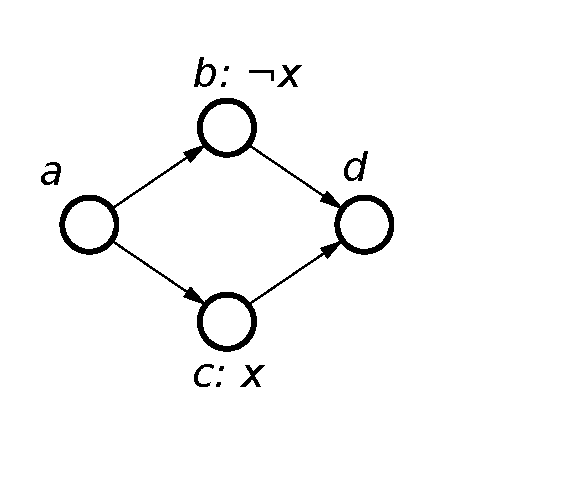
\includegraphics[scale=0.5]{fig/cpog_example}\hfill{}
\end{centering}

\end{frame}

\begin{frame}{Parametrised Graph Algebra}
PG Algebra is a generalisation of CPOGs

\begin{itemize}
\item Arbitrary set together with algebraic operations on it
\item Equivalence relation satisfying certain laws
\end{itemize}

\begin{figure}[h]
\begin{centering}
\hfill{}\subfloat[$G_{1} = a \seq b + c$]{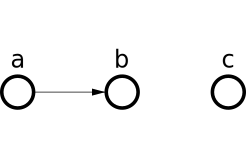
\includegraphics[scale=0.35]{fig/graph_3}
}\hfill{}\hfill{}\subfloat[$G_{2} = d$]{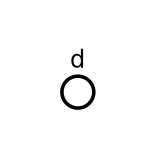
\includegraphics[scale=0.35]{fig/graph_4}
}\hfill{}\hfill{}\subfloat[$G_{1}+G_{2}$]{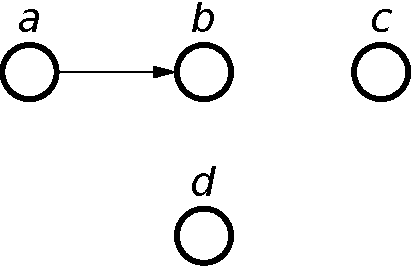
\includegraphics[scale=0.35]{fig/graph_overlay_3_4}
}\hfill{}\hfill{}\subfloat[$G_{1}\seq G_{2}$]{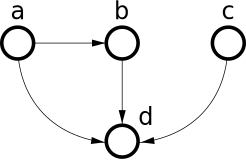
\includegraphics[scale=0.35]{fig/graph_sequence_3_4}
}\hfill{}
\par\end{centering}
\end{figure}
\end{frame}

\begin{frame}{Desired PG software support}
\begin{itemize}
\item Formula manipulations
\item Conversions to/from different formalisms
\item Hardware synthesis
\end{itemize}
\end{frame}
\begin{frame}{Formal methods}
\begin{itemize}
\item How do we know the theory is sound?
\item How do we know the tools are correct?
\item Need a way to statically ensure this.
\end{itemize}
\end{frame}
\begin{frame}{Agda}
Why Agda?
\begin{itemize}
\item A total functional programming language
\item A proof environment based on Curry-Howard isomorphism
\item Easy to learn when you know Haskell
\item Newbie-friendly community
\end{itemize}
\end{frame}

\begin{frame}{Graph Algebra}


\small{

\begin{hscode}\SaveRestoreHook
\column{B}{@{}>{\hspre}l<{\hspost}@{}}%
\column{3}{@{}>{\hspre}l<{\hspost}@{}}%
\column{17}{@{}>{\hspre}l<{\hspost}@{}}%
\column{29}{@{}>{\hspre}l<{\hspost}@{}}%
\column{E}{@{}>{\hspre}l<{\hspost}@{}}%
\>[B]{}\mathbf{record}\;\D{GraphOps}\;(\D{G}\;\D{B}\;\mathbin{:}\;\I{Set})\;\mathbin{:}\;\I{Set}\;\mathbf{where}{}\<[E]%
\\
\>[B]{}\mathbf{field}{}\<[E]%
\\
\>[B]{}\hsindent{3}{}\<[3]%
\>[3]{}\D{\varepsilon}\;\mathbin{:}\;\D{G}{}\<[E]%
\\
\>[B]{}\hsindent{3}{}\<[3]%
\>[3]{}\_\D{+}\_\;\mathbin{:}\;\D{G}\;\Varid{→}\;\D{G}\;\Varid{→}\;\D{G}{}\<[E]%
\\
\>[B]{}\hsindent{3}{}\<[3]%
\>[3]{}\_\D{\seq}\_\;\mathbin{:}\;\D{G}\;\Varid{→}\;\D{G}\;\Varid{→}\;\D{G}{}\<[E]%
\\[\blanklineskip]%
\>[B]{}\mathbf{record}\;\D{IsGraphAlgebra}\;\mathbin{:}\;\I{Set}\;\mathbf{where}{}\<[E]%
\\
\>[B]{}\mathbf{field}{}\<[E]%
\\
\>[B]{}\hsindent{3}{}\<[3]%
\>[3]{}\D{+assoc}\;{}\<[17]%
\>[17]{}\mathbin{:}\;\Varid{∀}\;\{\mskip1.5mu \Varid{p}\;\Varid{q}\;\Varid{r}\mskip1.5mu\}\;\Varid{→}\;(\Varid{p}\;\D{+}\;\Varid{q})\;\D{+}\;\Varid{r}\;\D{≈}\;\Varid{p}\;\D{+}\;(\Varid{q}\;\D{+}\;\Varid{r}){}\<[E]%
\\
\>[B]{}\hsindent{3}{}\<[3]%
\>[3]{}\D{+comm}\;{}\<[17]%
\>[17]{}\mathbin{:}\;\Varid{∀}\;\{\mskip1.5mu \Varid{p}\;\Varid{q}\mskip1.5mu\}\;{}\<[29]%
\>[29]{}\Varid{→}\;\Varid{p}\;\D{+}\;\Varid{q}\;\D{≈}\;\Varid{q}\;\D{+}\;\Varid{p}{}\<[E]%
\\
\>[B]{}\hsindent{3}{}\<[3]%
\>[3]{}\D{\seq{}assoc}\;{}\<[17]%
\>[17]{}\mathbin{:}\;\Varid{∀}\;\{\mskip1.5mu \Varid{p}\;\Varid{q}\;\Varid{r}\mskip1.5mu\}\;\Varid{→}\;(\Varid{p}\;\D{\seq}\;\Varid{q})\;\D{\seq}\;\Varid{r}\;\D{≈}\;\Varid{p}\;\D{\seq}\;(\Varid{q}\;\D{\seq}\;\Varid{r}){}\<[E]%
\\
\>[B]{}\hsindent{3}{}\<[3]%
\>[3]{}\D{\seq{}identity^l}\;{}\<[17]%
\>[17]{}\mathbin{:}\;\Varid{∀}\;\{\mskip1.5mu \Varid{p}\mskip1.5mu\}\;{}\<[29]%
\>[29]{}\Varid{→}\;\D{\varepsilon}\;\D{\seq}\;\Varid{p}\;\D{≈}\;\Varid{p}{}\<[E]%
\\
\>[B]{}\hsindent{3}{}\<[3]%
\>[3]{}\D{\seq{}identity^r}\;{}\<[17]%
\>[17]{}\mathbin{:}\;\Varid{∀}\;\{\mskip1.5mu \Varid{p}\mskip1.5mu\}\;{}\<[29]%
\>[29]{}\Varid{→}\;\Varid{p}\;\D{\seq}\;\D{\varepsilon}\;\D{≈}\;\Varid{p}{}\<[E]%
\\
\>[B]{}\hsindent{3}{}\<[3]%
\>[3]{}\D{distrib^l}\;{}\<[17]%
\>[17]{}\mathbin{:}\;\Varid{∀}\;\{\mskip1.5mu \Varid{p}\;\Varid{q}\;\Varid{r}\mskip1.5mu\}\;\Varid{→}\;\Varid{p}\;\D{\seq}\;(\Varid{q}\;\D{+}\;\Varid{r})\;\D{≈}\;\Varid{p}\;\D{\seq}\;\Varid{q}\;\D{+}\;\Varid{p}\;\D{\seq}\;\Varid{r}{}\<[E]%
\\
\>[B]{}\hsindent{3}{}\<[3]%
\>[3]{}\D{distrib^r}\;{}\<[17]%
\>[17]{}\mathbin{:}\;\Varid{∀}\;\{\mskip1.5mu \Varid{p}\;\Varid{q}\;\Varid{r}\mskip1.5mu\}\;\Varid{→}\;(\Varid{p}\;\D{+}\;\Varid{q})\;\D{\seq}\;\Varid{r}\;\D{≈}\;\Varid{p}\;\D{\seq}\;\Varid{r}\;\D{+}\;\Varid{q}\;\D{\seq}\;\Varid{r}{}\<[E]%
\\
\>[B]{}\hsindent{3}{}\<[3]%
\>[3]{}\D{decomposition}\;\mathbin{:}\;\Varid{∀}\;\{\mskip1.5mu \Varid{p}\;\Varid{q}\;\Varid{r}\mskip1.5mu\}\;\Varid{→}\;\Varid{p}\;\D{\seq}\;\Varid{q}\;\D{\seq}\;\Varid{r}\;\D{≈}\;\Varid{p}\;\D{\seq}\;\Varid{q}\;\D{+}\;\Varid{p}\;\D{\seq}\;\Varid{r}\;\D{+}\;\Varid{q}\;\D{\seq}\;\Varid{r}{}\<[E]%
\ColumnHook
\end{hscode}\resethooks
}
\end{frame}

\begin{frame}{Introducing conditions}
\begin{hscode}\SaveRestoreHook
\column{B}{@{}>{\hspre}l<{\hspost}@{}}%
\column{3}{@{}>{\hspre}l<{\hspost}@{}}%
\column{E}{@{}>{\hspre}l<{\hspost}@{}}%
\>[3]{}\D{[}\_\D{]}\_\;\mathbin{:}\;\D{B}\;\Varid{→}\;\D{G}\;\Varid{→}\;\D{G}{}\<[E]%
\ColumnHook
\end{hscode}\resethooks


\begin{hscode}\SaveRestoreHook
\column{B}{@{}>{\hspre}l<{\hspost}@{}}%
\column{3}{@{}>{\hspre}l<{\hspost}@{}}%
\column{56}{@{}>{\hspre}l<{\hspost}@{}}%
\column{59}{@{}>{\hspre}l<{\hspost}@{}}%
\column{E}{@{}>{\hspre}l<{\hspost}@{}}%
\>[3]{}\D{boolean\hyp{}algebra}\;\mathbin{:}\;\Conid{BooleanAlgebra}\;\D{B}{}\<[E]%
\\
\>[3]{}\D{true\hyp{}condition}\;\mathbin{:}\;\Varid{∀}\;\Varid{x}\;\Varid{→}\;[\mskip1.5mu \Varid{⊤}\mskip1.5mu]\;\Varid{x}\;\D{≈}\;\Varid{x}{}\<[E]%
\\
\>[3]{}\D{false\hyp{}condition}\;\mathbin{:}\;\Varid{∀}\;\Varid{x}\;\Varid{→}\;[\mskip1.5mu \Varid{⊥}\mskip1.5mu]\;\Varid{x}\;\D{≈}\;\D{\varepsilon}{}\<[E]%
\\
\>[3]{}\D{and\hyp{}condition}\;\mathbin{:}\;\Varid{∀}\;\Varid{f}\;\Varid{g}\;\Varid{x}\;\Varid{→}\;[\mskip1.5mu \Varid{f}\;\Varid{∧}\;\Varid{g}\mskip1.5mu]\;\Varid{x}\;\D{≈}\;[\mskip1.5mu \Varid{f}\mskip1.5mu]\;[\mskip1.5mu \Varid{g}\mskip1.5mu]\;{}\<[56]%
\>[56]{}\Varid{x}{}\<[E]%
\\
\>[3]{}\D{or\hyp{}condition}\;\mathbin{:}\;\Varid{∀}\;\Varid{f}\;\Varid{g}\;\Varid{x}\;\Varid{→}\;[\mskip1.5mu \Varid{f}\;\Varid{∨}\;\Varid{g}\mskip1.5mu]\;\Varid{x}\;\D{≈}\;[\mskip1.5mu \Varid{f}\mskip1.5mu]\;\Varid{x}\;\D{+}\;[\mskip1.5mu \Varid{g}\mskip1.5mu]\;{}\<[59]%
\>[59]{}\Varid{x}{}\<[E]%
\\
\>[3]{}\D{conditional+}\;\mathbin{:}\;\Varid{∀}\;\Varid{f}\;\Varid{x}\;\Varid{y}\;\Varid{→}\;[\mskip1.5mu \Varid{f}\mskip1.5mu]\;(\Varid{x}\;\D{+}\;\Varid{y})\;\D{≈}\;[\mskip1.5mu \Varid{f}\mskip1.5mu]\;\Varid{x}\;\D{+}\;[\mskip1.5mu \Varid{f}\mskip1.5mu]\;\Varid{y}{}\<[E]%
\\
\>[3]{}\D{conditional\!\seq}\;\mathbin{:}\;\Varid{∀}\;\Varid{f}\;\Varid{x}\;\Varid{y}\;\Varid{→}\;[\mskip1.5mu \Varid{f}\mskip1.5mu]\;(\Varid{x}\;\D{\seq}\;\Varid{y})\;\D{≈}\;[\mskip1.5mu \Varid{f}\mskip1.5mu]\;\Varid{x}\;\D{\seq}\;[\mskip1.5mu \Varid{f}\mskip1.5mu]\;\Varid{y}{}\<[E]%
\ColumnHook
\end{hscode}\resethooks
\end{frame}

\begin{frame}{PG Algebra theorems}

The following theorems has been derived from the axioms:





\begin{hscode}\SaveRestoreHook
\column{B}{@{}>{\hspre}l<{\hspost}@{}}%
\column{3}{@{}>{\hspre}l<{\hspost}@{}}%
\column{E}{@{}>{\hspre}l<{\hspost}@{}}%
\>[B]{}\D{+identity}\;\mathbin{:}\;\Varid{∀}\;\Varid{p}\;\Varid{→}\;\Varid{p}\;\D{+}\;\D{\varepsilon}\;\D{≈}\;\Varid{p}{}\<[E]%
\\[\blanklineskip]%
\>[B]{}\D{+idempotence}\;\mathbin{:}\;\Varid{∀}\;\Varid{p}\;\Varid{→}\;\Varid{p}\;\D{+}\;\Varid{p}\;\D{≈}\;\Varid{p}{}\<[E]%
\\[\blanklineskip]%
\>[B]{}\D{absorption^l}\;\mathbin{:}\;\Varid{∀}\;\Varid{p}\;\Varid{q}\;\Varid{→}\;\Varid{p}\;\D{\seq}\;\Varid{q}\;\D{+}\;\Varid{p}\;\D{≈}\;\Varid{p}\;\D{\seq}\;\Varid{q}{}\<[E]%
\\[\blanklineskip]%
\>[B]{}\D{absorption^r}\;\mathbin{:}\;\Varid{∀}\;\Varid{p}\;\Varid{q}\;\Varid{→}\;\Varid{p}\;\D{\seq}\;\Varid{q}\;\D{+}\;\Varid{q}\;\D{≈}\;\Varid{p}\;\D{\seq}\;\Varid{q}{}\<[E]%
\\[\blanklineskip]%
\>[B]{}\D{choice\hyp{}propagation_1}\;\mathbin{:}\;\Varid{∀}\;\Varid{b}\;\Varid{p}\;\Varid{q}\;\Varid{r}\;\Varid{→}\;{}\<[E]%
\\
\>[B]{}\hsindent{3}{}\<[3]%
\>[3]{}\D{[}\Varid{b}\D{]}\;(\Varid{p}\;\D{\seq}\;\Varid{q})\;\D{+}\;\D{[}\D{¬}\;\Varid{b}\D{]}\;(\Varid{p}\;\D{\seq}\;\Varid{r})\;\D{≈}\;\Varid{p}\;\D{\seq}\;(\D{[}\Varid{b}\D{]}\;\Varid{q}\;\D{+}\;\D{[}\D{¬}\;\Varid{b}\D{]}\;\Varid{r}){}\<[E]%
\\[\blanklineskip]%
\>[B]{}\D{choice\hyp{}propagation_2}\;\mathbin{:}\;\Varid{∀}\;\Varid{b}\;\Varid{p}\;\Varid{q}\;\Varid{r}\;\Varid{→}\;{}\<[E]%
\\
\>[B]{}\hsindent{3}{}\<[3]%
\>[3]{}\D{[}\Varid{b}\D{]}\;(\Varid{p}\;\D{\seq}\;\Varid{r})\;\D{+}\;\D{[}\D{¬}\;\Varid{b}\D{]}\;(\Varid{q}\;\D{\seq}\;\Varid{r})\;\D{≈}\;(\D{[}\Varid{b}\D{]}\;\Varid{p}\;\D{+}\;\D{[}\D{¬}\;\Varid{b}\D{]}\;\Varid{q})\;\D{\seq}\;\Varid{r}{}\<[E]%
\\[\blanklineskip]%
\>[B]{}\D{condition\hyp{}regularisation}\;\mathbin{:}\;\Varid{∀}\;\Varid{f}\;\Varid{g}\;\Varid{p}\;\Varid{q}\;\Varid{→}\;{}\<[E]%
\\
\>[B]{}\hsindent{3}{}\<[3]%
\>[3]{}\D{[}\Varid{f}\D{]}\;\Varid{p}\;\D{\seq}\;\D{[}\Varid{g}\D{]}\;\Varid{q}\;\D{≈}\;\D{[}\Varid{f}\D{]}\;\Varid{p}\;\D{+}\;\D{[}\Varid{g}\D{]}\;\Varid{q}\;\D{+}\;\D{[}\Varid{f}\;\D{∧}\;\Varid{g}\D{]}\;(\Varid{p}\;\D{\seq}\;\Varid{q}){}\<[E]%
\ColumnHook
\end{hscode}\resethooks
\end{frame}














\begin{frame}{Formula data structure}

Formula data structure mimics the algebra operations:

\begin{hscode}\SaveRestoreHook
\column{B}{@{}>{\hspre}l<{\hspost}@{}}%
\column{3}{@{}>{\hspre}l<{\hspost}@{}}%
\column{E}{@{}>{\hspre}l<{\hspost}@{}}%
\>[B]{}\mathbf{data}\;\D{PGFormula}\;\D{B}\;\D{V}\;\mathbin{:}\;\I{Set}\;\mathbf{where}{}\<[E]%
\\
\>[B]{}\hsindent{3}{}\<[3]%
\>[3]{}\_\C{+}\_\;\mathbin{:}\;(\Varid{x}\;\Varid{y}\;\mathbin{:}\;\D{PGFormula})\;\Varid{→}\;\D{PGFormula}{}\<[E]%
\\
\>[B]{}\hsindent{3}{}\<[3]%
\>[3]{}\_\C{\seq}\_\;\mathbin{:}\;(\Varid{x}\;\Varid{y}\;\mathbin{:}\;\D{PGFormula})\;\Varid{→}\;\D{PGFormula}{}\<[E]%
\\
\>[B]{}\hsindent{3}{}\<[3]%
\>[3]{}\C{ε}\;\mathbin{:}\;\D{PGFormula}{}\<[E]%
\\
\>[B]{}\hsindent{3}{}\<[3]%
\>[3]{}\C{var}\;\mathbin{:}\;(\Varid{a}\;\mathbin{:}\;\D{V})\;\Varid{→}\;\D{PGFormula}{}\<[E]%
\\
\>[B]{}\hsindent{3}{}\<[3]%
\>[3]{}\C{[}\anonymous \C{]}\;\anonymous \;\mathbin{:}\;(\Varid{c}\;\mathbin{:}\;\D{B})\;\Varid{→}\;\D{PGFormula}\;\Varid{→}\;\D{PGFormula}{}\<[E]%
\ColumnHook
\end{hscode}\resethooks
\end{frame}

\begin{frame}{Making sense of the formulae}

We need to give the formula semantics in terms of algebra.

\begin{hscode}\SaveRestoreHook
\column{B}{@{}>{\hspre}l<{\hspost}@{}}%
\column{5}{@{}>{\hspre}l<{\hspost}@{}}%
\column{E}{@{}>{\hspre}l<{\hspost}@{}}%
\>[B]{}\D{pg\hyp{}eval}\;\mathbin{:}\;\D{PGFormula}\;\D{B}\;\D{V}\;{}\<[E]%
\\
\>[B]{}\hsindent{5}{}\<[5]%
\>[5]{}\Varid{→}\;(\D{V}\;\Varid{→}\;\D{G})\;\Varid{→}\;\Conid{PGAlgebra}\;\D{G}\;\D{V}\;{}\<[E]%
\\
\>[B]{}\hsindent{5}{}\<[5]%
\>[5]{}\Varid{→}\;\D{G}{}\<[E]%
\ColumnHook
\end{hscode}\resethooks
\begin{hscode}\SaveRestoreHook
\column{B}{@{}>{\hspre}l<{\hspost}@{}}%
\column{10}{@{}>{\hspre}l<{\hspost}@{}}%
\column{E}{@{}>{\hspre}l<{\hspost}@{}}%
\>[B]{}\_\D{≈_{f}}\_\;\mathbin{:}\;\Varid{∀}\;\D{B}\;\D{V}\;\Varid{→}\;\D{PGFormula}\;\D{B}\;\D{V}\;\Varid{→}\;\D{PGFormula}\;\D{B}\;\D{V}\;\Varid{→}\;\I{Set}{}\<[E]%
\\
\>[B]{}\Varid{a}\;\D{≈_{f}}\;\Varid{b}\;\mathrel{=}\;\Varid{∀}\;\Varid{assign}\;\Varid{alg}\;{}\<[E]%
\\
\>[B]{}\hsindent{10}{}\<[10]%
\>[10]{}\Varid{→}\;\D{pg\hyp{}eval}\;\Varid{a}\;\Varid{assign}\;\Varid{alg}\;\D{≈}\;\D{pg\hyp{}eval}\;\Varid{b}\;\Varid{assing}\;\Varid{alg}{}\<[E]%
\ColumnHook
\end{hscode}\resethooks

\end{frame}

\begin{frame}{PG Formula normal form}

\begin{hscode}\SaveRestoreHook
\column{B}{@{}>{\hspre}l<{\hspost}@{}}%
\column{E}{@{}>{\hspre}l<{\hspost}@{}}%
\>[B]{}\D{BF}\;\mathrel{=}\;\D{BoolFormula}\;\D{B}{}\<[E]%
\\
\>[B]{}\D{PG}\;\mathrel{=}\;\D{PGFormula}\;\D{BF}\;\D{V}{}\<[E]%
\\[\blanklineskip]%
\>[B]{}\D{Node}\;\mathrel{=}\;\D{V}\;\I{⊎}\;(\D{V}\;\I{×}\;\D{V}){}\<[E]%
\\
\>[B]{}\D{Lit}\;\mathrel{=}\;\D{Node}\;\I{×}\;\D{BF}{}\<[E]%
\\
\>[B]{}\D{NF}\;\mathrel{=}\;\I{List}\;\D{Lit}{}\<[E]%
\ColumnHook
\end{hscode}\resethooks

\begin{hscode}\SaveRestoreHook
\column{B}{@{}>{\hspre}l<{\hspost}@{}}%
\column{E}{@{}>{\hspre}l<{\hspost}@{}}%
\>[B]{}\D{fromNode}\;\mathbin{:}\;\D{Node}\;\Varid{→}\;\D{PG}{}\<[E]%
\\
\>[B]{}\D{fromNode}\;(\C{inj_1}\;\Varid{x})\;\mathrel{=}\;\C{var}\;\Varid{x}{}\<[E]%
\\
\>[B]{}\D{fromNode}\;(\C{inj_2}\;(\Varid{x}\C{,}\Varid{y}))\;\mathrel{=}\;\C{var}\;\Varid{x}\;\C{\seq}\;\C{var}\;\Varid{y}{}\<[E]%
\\[\blanklineskip]%
\>[B]{}\D{fromLit}\;\mathbin{:}\;\D{Lit}\;\Varid{→}\;\D{PG}{}\<[E]%
\\
\>[B]{}\D{fromLit}\;(\Varid{node}\C{,}\Varid{cond})\;\mathrel{=}\;\C{[}\Varid{cond}\C{]}\;\D{fromNode}\;\Varid{node}{}\<[E]%
\\[\blanklineskip]%
\>[B]{}\D{fromNF}\;\mathbin{:}\;\D{NF}\;\Varid{→}\;\D{PG}{}\<[E]%
\\
\>[B]{}\D{fromNF}\;\mathrel{=}\;\I{foldr}\;\_\C{+}\_\;\C{ε}\;\I{∘}\;\I{map}\;\D{fromLit}{}\<[E]%
\ColumnHook
\end{hscode}\resethooks

\end{frame}

\begin{frame}{PG Formula normalisation}

\begin{hscode}\SaveRestoreHook
\column{B}{@{}>{\hspre}l<{\hspost}@{}}%
\column{3}{@{}>{\hspre}l<{\hspost}@{}}%
\column{E}{@{}>{\hspre}l<{\hspost}@{}}%
\>[3]{}\D{fromNF}\;\mathbin{:}\;\D{NF}\;\Varid{→}\;\D{PG}{}\<[E]%
\\[\blanklineskip]%
\>[3]{}\D{normalise}\;\mathbin{:}\;\D{PG}\;\Varid{→}\;\D{NF}{}\<[E]%
\\
\>[3]{}\Varid{...}\;(\Varid{35}\;\Varid{lines}\;\Varid{of}\;\Varid{implementation}){}\<[E]%
\\[\blanklineskip]%
\>[3]{}\D{normalise\hyp{}correct}\;\mathbin{:}\;\Varid{∀}\;\Varid{f}\;\Varid{→}\;\Varid{f}\;\D{≈}\;\D{fromNF}\;(\D{normalise}\;\Varid{f}){}\<[E]%
\\
\>[3]{}\Varid{...}\;(\Varid{100}\;\Varid{lines}\;\Varid{of}\;\Varid{proof}){}\<[E]%
\ColumnHook
\end{hscode}\resethooks
\end{frame}

\begin{frame}{Conclusions}

\begin{itemize}
\item We have successfuly formalised the PG Algebra.
\item We have developed a simple verified program for converting formulae to normal forms.
\end{itemize}

\end{frame}

\end{document}
